\problemname{\problemyamlname}

On a small island far far away, a handful of old men live isolated from the rest of the world.
The entire island is divided into plots of land by fences, and each old man owns
a single plot of land bounded by fences on all sides. (The region
outside all fences is the ocean.)
Each of the inhabitants needs fish to survive and the only place where they can fish is the ocean surrounding them.
Since not every plot of land is connected to the ocean,
some of the men might need to pass through the land of others before being able to fish.
The men can cross a single fence at a time, but cannot go through fenceposts or
locations where fences intersect.

Unfortunately, the old men are greedy.
They demand one fish each time a person wants to enter their land.
Since they do not want to lose too much fish to the others,
every old man chooses a route that minimizes the number of fish he has to pay to get to the ocean.

Over the years, this has led to rivalry between the old men.
Each man hates all other men who have to pay less than him to reach the ocean.
Two men only \emph{like} each other if they have to pay the same amount of fish to reach the ocean.

\begin{figure}[h]
  \centering
  \hfill
  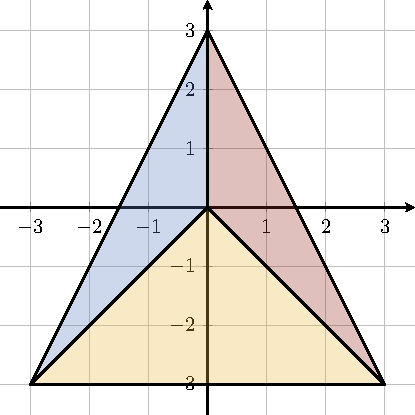
\includegraphics[height=3.5cm]{sample1.pdf}
  \hfill
  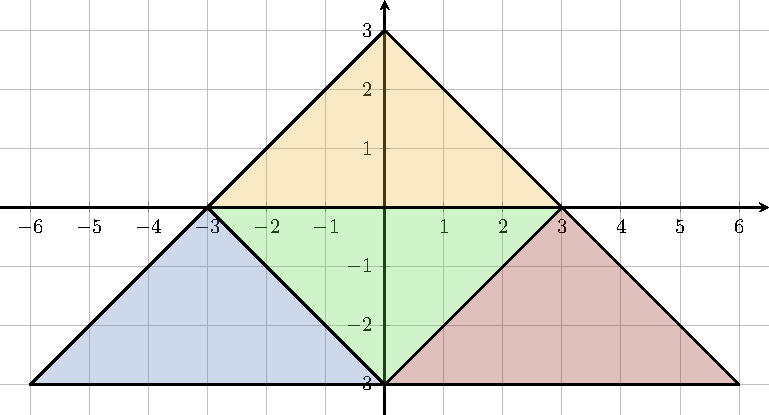
\includegraphics[height=3.5cm]{sample2.pdf}
  \hfill
  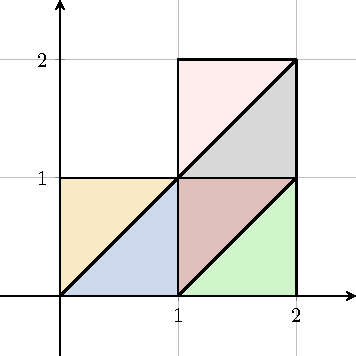
\includegraphics[height=3.5cm]{sample3.pdf}
  \hfill
  \hfill
  \caption{
    Illustrations of the first three Sample Inputs.
    In Sample Input 1, every man has direct access to the ocean, so they all like each other.
    In Sample Input 2, there does not exist a pair of neighbours who like each other,
    because the man living in the middle needs to pay one fish,
    whereas all of his neighbours do not have to pay any fish to reach the ocean.
    In Sample Input 3, there are six men, some of whom are friendly neighbours.
  }
  \label{fig:islands}
\end{figure}

The natural question which now occurs is:
are there some old men on this island who are neighbours (owning land on
opposite sides of a single fence) and like each other?
See Figure~\ref{fig:islands} for two islands with opposite answers to this question.

\begin{Input}
  The input consists of:
  \begin{itemize}
    \item One line with an integer $n$ ($3 \le n \le 1000$), the number of fences.
    \item $n$ lines, each with four integers $x_1$, $y_1$, $x_2$, and $y_2$
  ($\left|x_1\right|, \left|y_1\right|, \left|x_2\right|, \left|y_2\right|\leq 10^6$, $(x_1,y_1)\neq(x_2,y_2)$), indicating a straight fence between
  fenceposts at $(x_1,y_1)$ and $(x_2, y_2)$.
  \end{itemize}

  Note that fences may intersect internally, and that three or more fences may intersect in the same location.

  It is guaranteed that any two fences intersect only in at most one point.
  Furthermore, after crossing a single fence, one always ends up in a different region.
  All regions together form a single island, where any region can be reached from any other region.
\end{Input}

\begin{Output}
  If there exists a pair of neighbours who like each other, then output
  ``\texttt{yes}''. Otherwise, output ``\texttt{no}''.
\end{Output}
